\documentclass[12pt]{article}
\usepackage{graphicx}

\begin{document}

Andrew Brandt
8-28-2022

\Large 01 Puzzle 1 - Jungle Roads, A Warm Up Puzzle 

\normalsize

\vspace{5mm} %5mm vertical space

Four villages are located in a dense jungle with jungle all around everywhere, densely dense.
Curiously, they are each within Verizon’s 5G coverage area so the village elders have used their
M1 iPads to access Google Earth and have noticed that the four villages, named W, X, Y and Z,
seem to be at the vertices of a square, in that order, with sides of length S kilometers.

\vspace{5mm}

Immediately a committee is formed to construct a road system connecting the villages and you
are appointed to the committee as a junior member. The directive from the village elders is to
construct a road system that allows any villager to somehow get from any village to any other
village over these roads but which minimizes the destruction of the precious jungle environment.
The chair of the committee, a powerful and easily upset warrior with a fierce temper and many
sharp weapons, but who is otherwise a reasonable fellow, proposes that they just “Complete the
Square”, that is, build roads around the edge of the square with a total length of 4 * S kilometers.

\vspace{5mm}

\noindent{What say you?}

\vspace{10mm}

\noindent
To start I am going to make some assumptions on this puzzle.
The first is that the villages are in a perfect square. That is, they are always evenly spaced apart.
The next assumption that I am going to make is that there is always a shorter path than just completing the square.

\vspace{5mm}
\noindent
My first idea here is to simply always remove one side of the square.
This would always still leave a complete path to every village but would take the distace from 4s down to 3s.
This method also scales for any number of villages as long as its greater than 2.

\vspace{5mm}
\noindent
The next idea is one that only requires building two paths crossing over each other.
This method brings down the distance significantly compared to 4s.
The downside to this method is that it might not scale as well when there are more than 4 villages to connect.


\vspace{5mm}

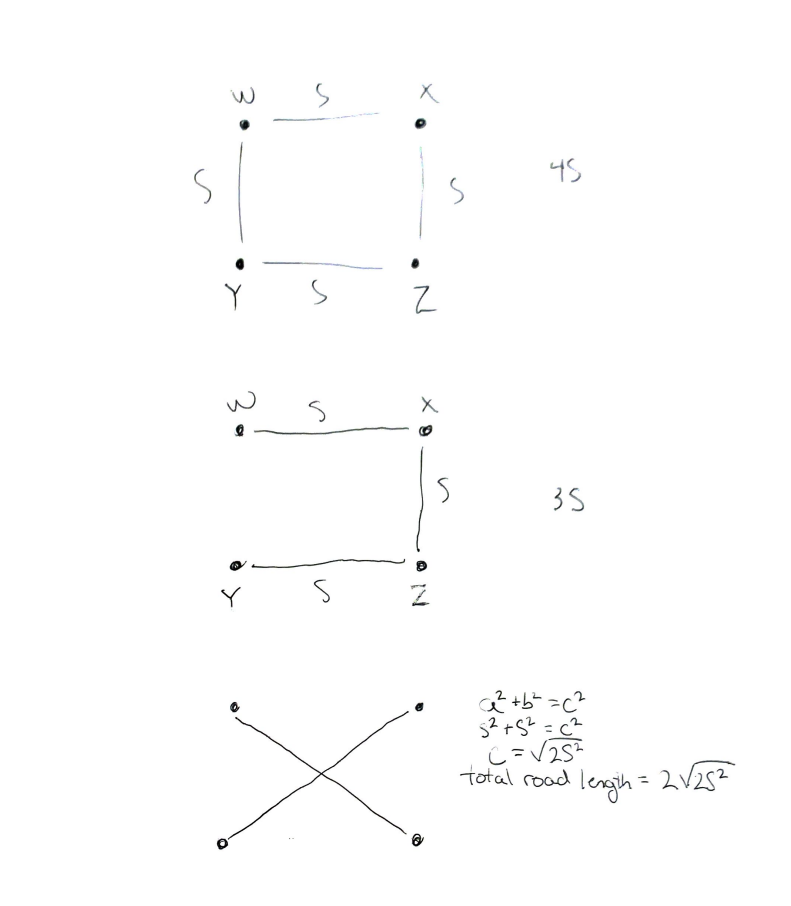
\includegraphics[scale=.75]{table1}

\vspace{5mm}

The trend I am seeing here is to join all the points in the middle. Though I think it depends on the number of villages.
With 4, only half the amount of lines need to be drawn compared to just the 4s solution. Given these lines are longer than s, they will be shorter than 2s.
When there is an odd number of villages, more lines will need to be drawn than just the number of villages/2.

\vspace{5mm}

The solution to follow this trend spotted is to connect the points that are directly oposite for an even number of villages
If there is an odd number of villages, connecting a village with one of the most directly opposite points should work.
Also for odd numbers of villages, because the lines drawn acros will have some overlap, if the is space in the middle between two crossing lines, the space does not need a line through it.


\end{document}